\documentclass[a0paper,portrait]{baposter}


\usepackage{minipage-marginpar}
\usepackage{wrapfig}
\usepackage{lmodern}
\usepackage{amsmath}
\usepackage[utf8]{inputenc} %unicode support
\usepackage[T1]{fontenc}
\usepackage{tcolorbox}
\usepackage{bm}
\selectcolormodel{cmyk}
\usepackage[font=scriptsize]{caption}
\usepackage{enumitem}

% \graphicspath{{figures/}} % Directory in which figures are stored

\newcommand{\compresslist}{%
\setlength{\itemsep}{0pt}%
\setlength{\parskip}{1pt}%
\setlength{\parsep}{0pt}%
}

\renewcommand{\baselinestretch}{1}

\newenvironment{boenumerate}
  {\begin{enumerate}\renewcommand\labelenumi{\textbf\theenumi.}}
  {\end{enumerate}}

\usepackage{tikz}
\newcommand*\circled[1]{\tikz[baseline=(char.base)]{
            \node[shape=circle,draw,inner sep=2pt] (char) {#1};}}

\begin{document}


\definecolor{darkblue}{cmyk}{0.78,0.78,0,0.56}
\definecolor{lightblue}{cmyk}{0.71,0.46,0,0.41}
\definecolor{silver}{cmyk}{0.08,0.07,0,0.02}

\newtcolorbox{outline}{colback=silver,colframe=darkblue,arc=10pt,
						enlarge top by=1px, enlarge bottom by=1px,
						grow to left by=-10px, grow to right by=-10px}

\newenvironment{myindentpar}[1]%
  {\begin{list}{}%
          {\setlength{\leftmargin}{#1}}%
          \item[]%
  }
  {\end{list}}



\begin{poster}
{
grid=false,
headerborder=open, % Adds a border around the header of content boxes
colspacing=1em, % Column spacing
bgColorOne=white, % Background color for the gradient on the left side of the poster
bgColorTwo=white, % Background color for the gradient on the right side of the poster
borderColor=darkblue, % Border color
headerColorOne=lightblue, % Background color for the header in the content boxes (left side)
headerColorTwo=lightblue, % Background color for the header in the content boxes (right side)
headerFontColor=white, % Text color for the header text in the content boxes
boxColorOne=white, % Background color of the content boxes
textborder=rounded, %rectangle, % Format of the border around content boxes, can be: none, bars, coils, triangles, rectangle, rounded, roundedsmall, roundedright or faded
eyecatcher=false, % Set to false for ignoring the left logo in the title and move the title left
headerheight=0.11\textheight, % Height of the header
headershape=rounded, % Specify the rounded corner in the content box headers, can be: rectangle, small-rounded, roundedright, roundedleft or rounded
headershade=plain,
headerfont=\Large\textsf, % Large, bold and sans serif font in the headers of content boxes
%textfont={\setlength{\parindent}{1.5em}}, % Uncomment for paragraph indentation
linewidth=2pt % Width of the border lines around content boxes
}
{}
%
%----------------------------------------------------------------------------------------
%	TITLE AND AUTHOR NAME
%----------------------------------------------------------------------------------------
%
{
\textsf %Sans Serif
{
\vspace{1em}\\
Technological Improvements or Climate Change? \\
\vspace{0.1mm}\\
\LARGE -- Bayesian Modeling of Time-Varying Conformance to Benford's Law. \\
}
} % Poster title
% {\vspace{1em} Marta Stepniewska, Pawel Siedlecki\\ % Author names
% {\small \vspace{0.7em} Department of Bioinformatics, Institute of Biochemistry and Biophysics, PAS, Warsaw, Pawinskiego 5a}} % Author email addresses
{\indent \sf Junho Lee* and Miguel de Carvalho
\vspace{0.5em}\\
\indent \normalsize{ School of Mathematics, University of Edinburgh, Edinburgh, U.K. \qquad \qquad\qquad \qquad  * j.lee-63@sms.ed.ac.uk}
%\vspace{0.2em}\\
%
}
{\vspace{3em}\\

\includegraphics[scale=0.9]{logo.jpg}} % University/lab logo

\renewcommand{\baselinestretch}{1.1}

\headerbox{1. Introduction}{name=introduction,column=0,row=0, span=3}{

\begin{wrapfigure}{r}{0.25\textwidth}
    \vspace{-10pt}
    \begin{center}
        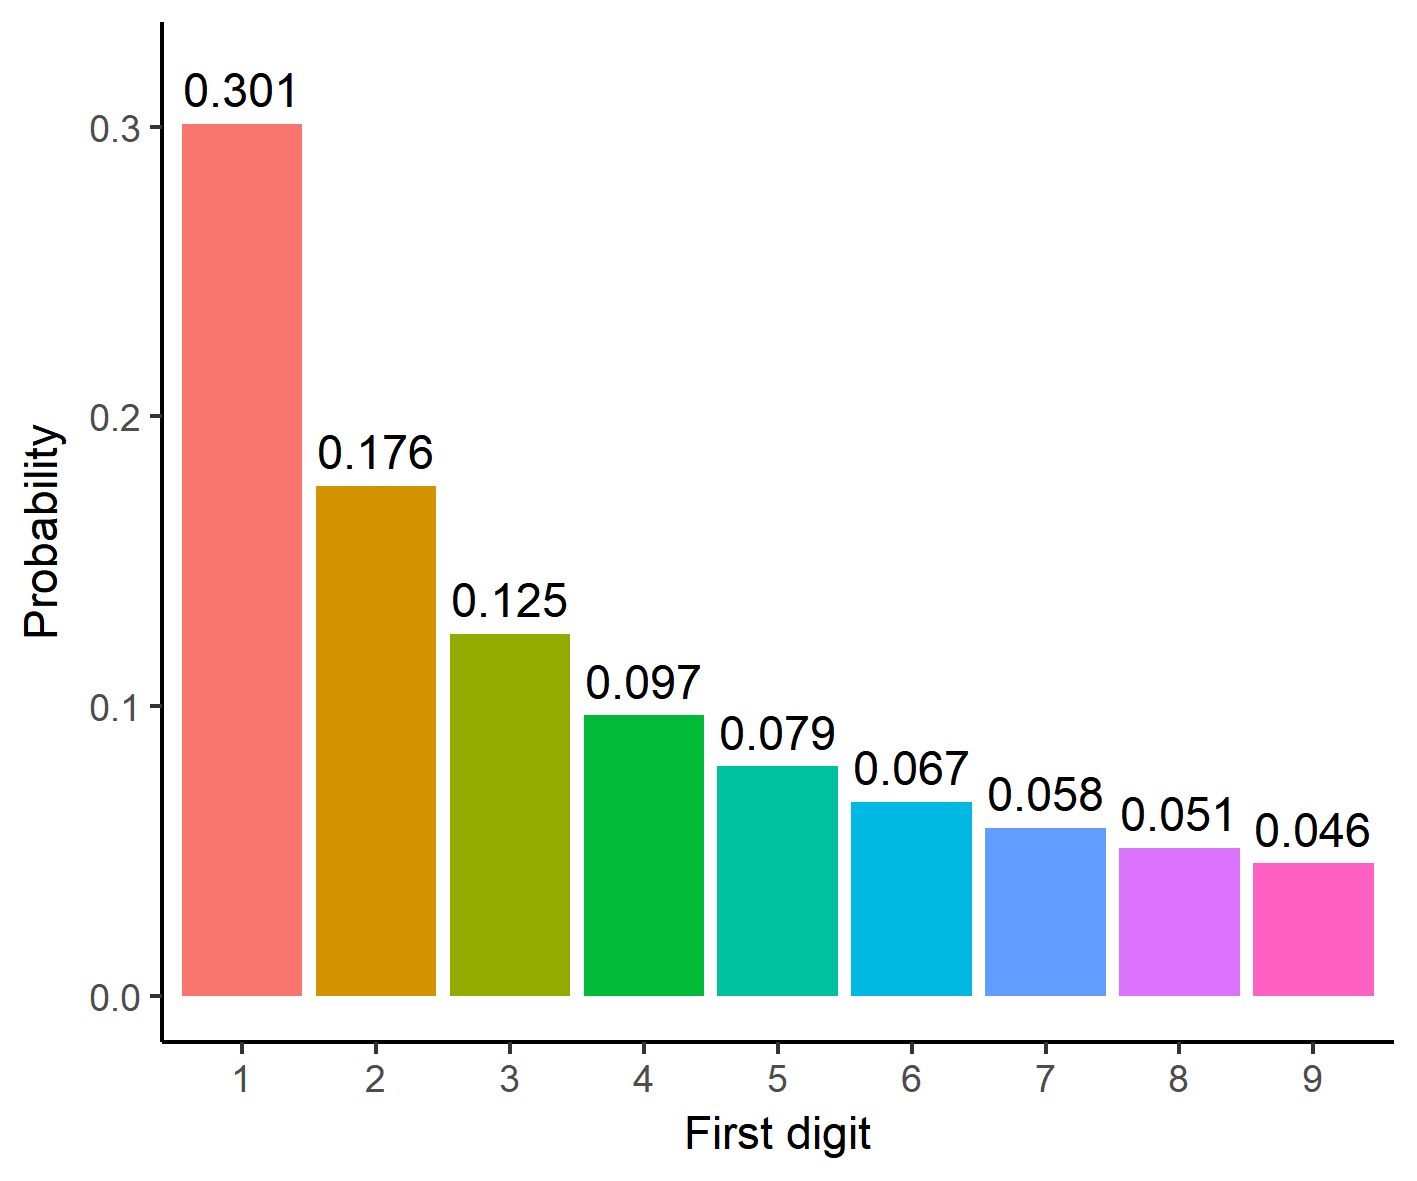
\includegraphics[width=0.8\linewidth]{Benford}
        
    \scriptsize Fig 1. \textbf{Benford's Law}\\ 
    \end{center}
    %\vspace{-145pt}
\end{wrapfigure}
Benford's Law is an empirical observation on the distribution of first digits of numerical data.  The law states that the frequency of the first digit of data follows a logarithmically decreasing distribution given by 
$$\textsf{p}_d=\textsf{P}(D=d)= \log_{10} \left(1+ \frac{1}{d}\right), \quad d=1,\ldots,9, \quad D: \;\text{ the first significant digit} $$
Benford's Law has been recently advocated as a natural tool to assess the quality and homogeneity of large datasets spanning several decades \cite{b_benford2}. 
This study develops a Bayesian time-varying model that tracks dynamics of the first-digit distribution and evaluates the compliance with the Benford's Law.   We apply the model to the global tropical cyclone data. Our goals are to (1) learn about the dynamics of the leading digits,  (2) examine conformance to Benford's Law, and  (3) assess the homogeneity within the dataset.


}

\headerbox{2. Model}{name=model,span=2,column=0,below=introduction}{ % To reduce this block to 1 column width, remove 'span=2'
\begin{itemize}
\item \textbf{(Multinomial Logistic Model)} Define $N_t$  as a total number of trials in time $t$ and $\bm{n}_t=(n_{1,t},\ldots,n_{9,t})$ as a random vector such that  each $n_{d,t}$ denotes a frequency of event that the first digit equals to $d$ during year $t$.
\item \textbf{(Penalized Splines)} For inference, we follow a Bayesian version of penalized spline approach \cite{LangBrezger2004,BrezgerSteiner2008} so as to learn about dynamics of first-digit probability.
\end{itemize}



\vspace{-0.3cm}
 \begin{outline}
        \textbf{Bayesian Smooth Multinomial Model}
$$\begin{aligned} 
\text{(Sampling distribution)}& \quad (n_{1,t} ,\ldots,n_{9,t})\sim \text{Mult}(N_t, p_{1,t},\ldots,p_{9,t}),\\ 
\text{(Model Specification)}&\quad p_{d,t}= \frac{\exp(\eta_{d,t})}{1+\sum_{d=1}^8 \exp(\eta_{d,t})},\quad p_{9,t}= \frac{1}{1+\sum_{d=1}^8 \exp(\eta_{d,t})},\\
&\quad \eta_{d,t} = \sum_{k=1}^{K+3} \beta_{d,k} B_{d,k}(t),\\
\text{(Random Walk Prior)}& \quad \beta_{1,d} \sim  U(c_0,d_0), \quad \beta_{k+1,d} = \beta_{k,d} + \varepsilon_d, \quad  \varepsilon_d \sim N(0,\tau_d^2), \\
\text{(Hyper-Prior)}& \quad \tau_d^2 \sim \text{IG}(a_0,b_0). \\
\end{aligned}$$
\end{outline}
}




\renewcommand{\baselinestretch}{1.1}

\headerbox{3. Data}{name=application,column=2,below=introduction,span=1}{
\begin{myindentpar}{0.1cm}
The Global Tropical Cyclone (GTC) dataset includes a register of tropical cyclones around the world since 1842. The dataset
\end{myindentpar}
\begin{itemize}[leftmargin=0.5cm]
\vspace{-0.5cm}
\item provides information on a geographical location, frequency, and intensity of each cyclone.
\item stimulates a debate on the quality of early records for assessing the influence of climate change on the occurrence of cyclones \cite{Joannes2015}.
\end{itemize}
\begin{center}
\vspace{-0.2cm}
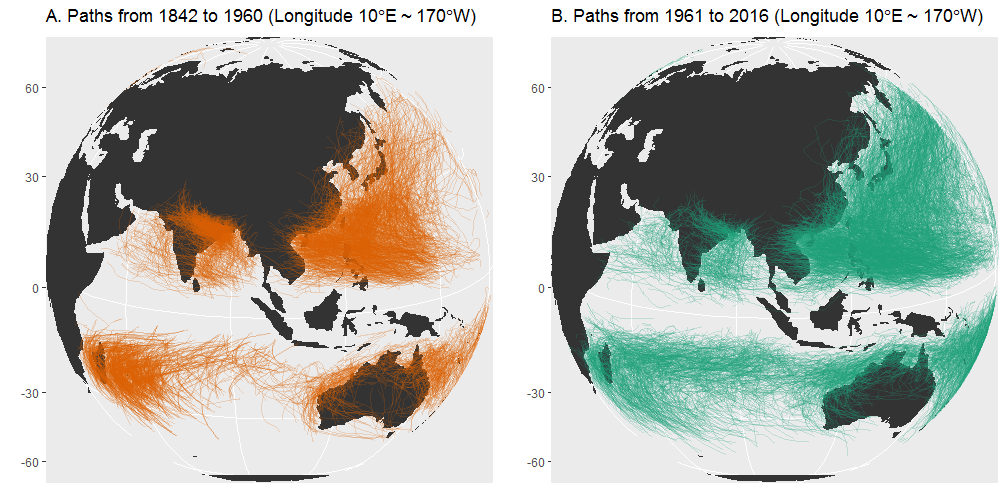
\includegraphics[width=1\linewidth]{Twomaps.png}

\scriptsize Fig 2. \textbf{Map of tropical cyclone tracks since 1842}\\ 
\end{center}

\vspace{-0.3cm}
\begin{myindentpar}{0.1cm}
We calculate a traveled distance of each cyclone and analyze the distribution of the leading digits of 12,741 cyclones until 2016.
\end{myindentpar}
\vspace{-0.3cm}
\begin{myindentpar}{0.1cm}
Th first-digit distribution of the pooled data resemble the probabilities from Benford’s Law.
\end{myindentpar}
\begin{flushleft}
\vspace{-0.2cm}
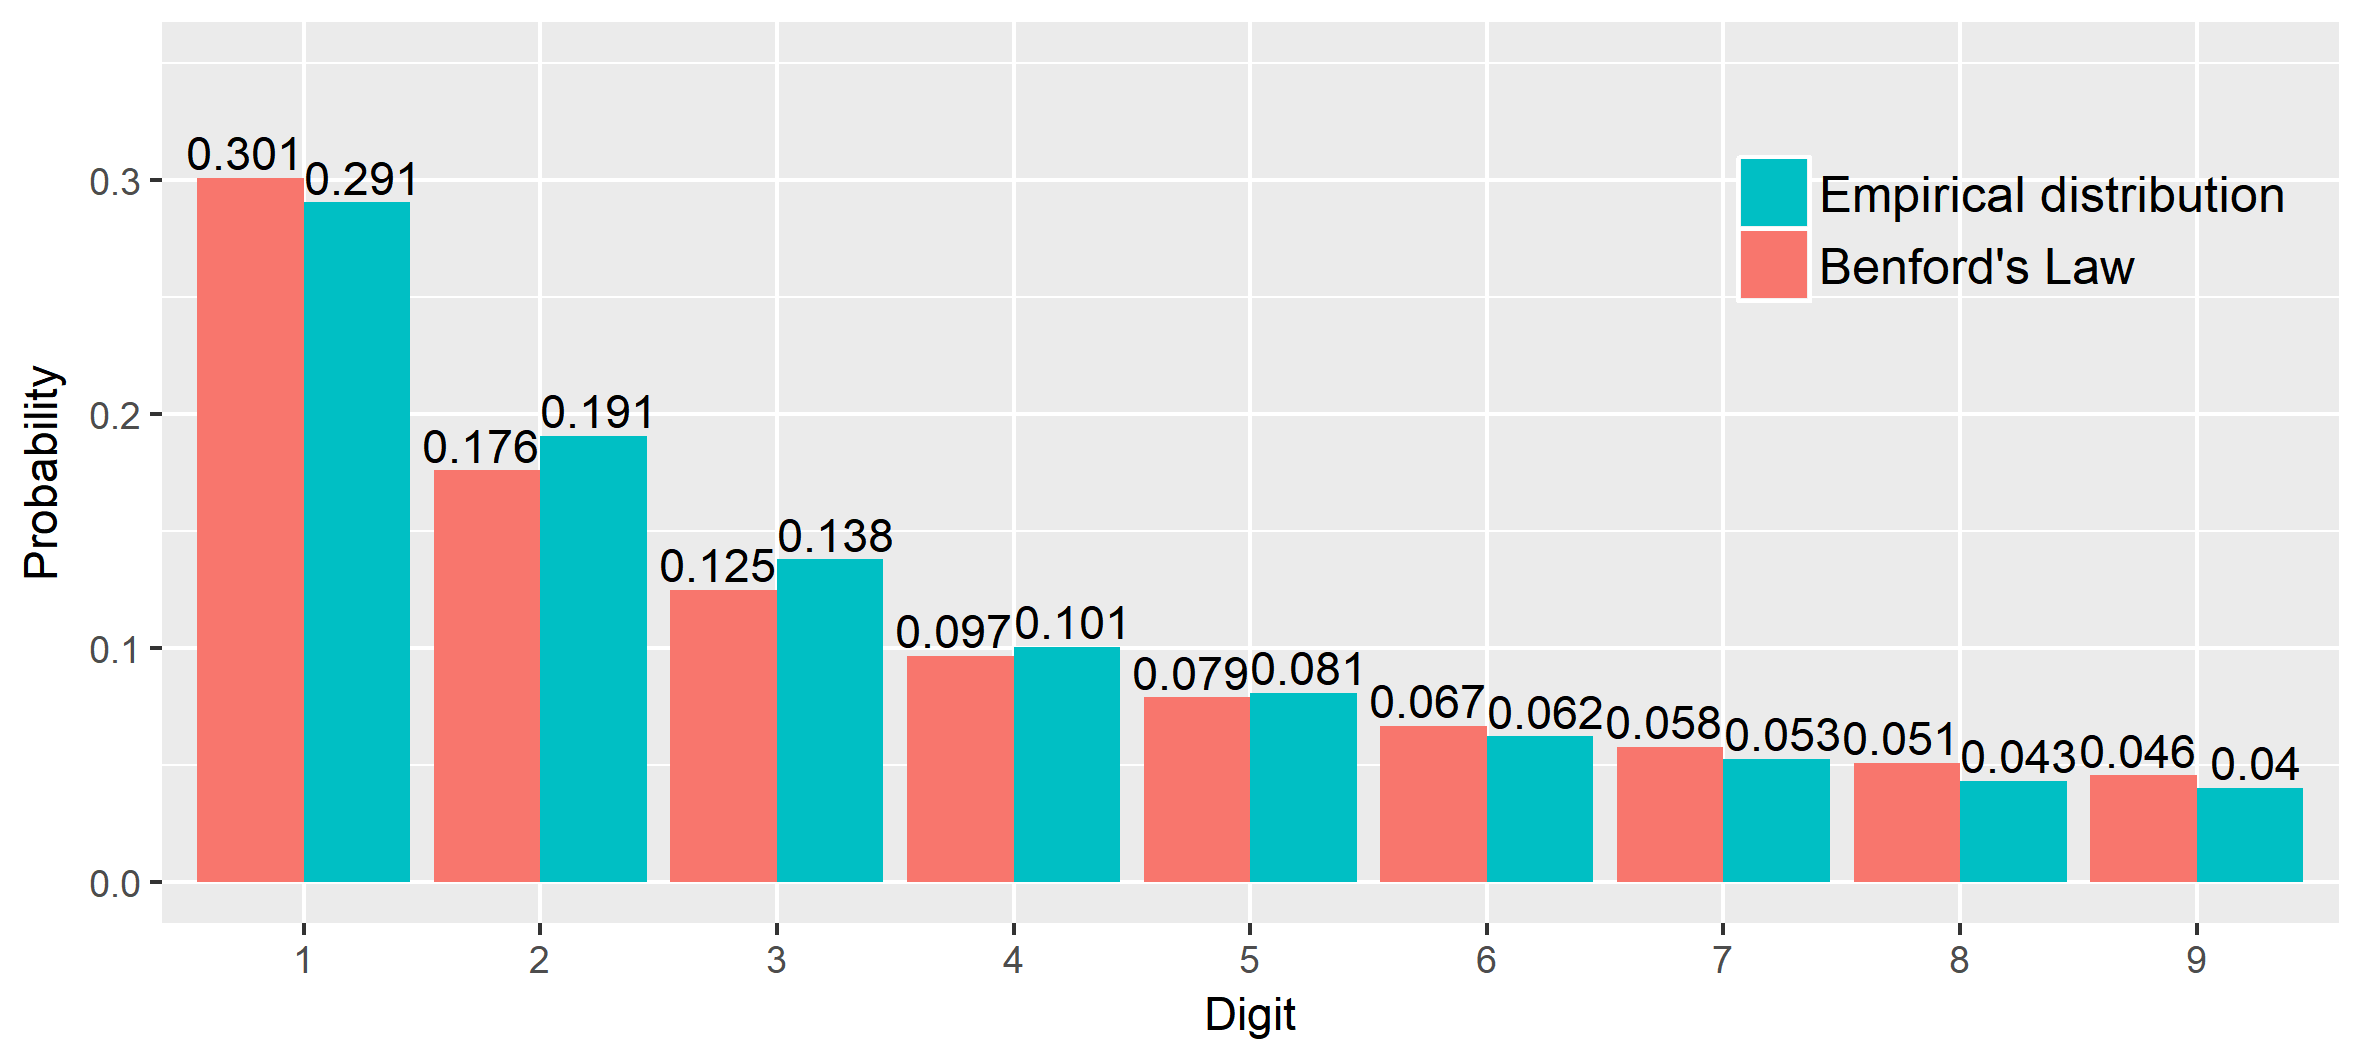
\includegraphics[width=0.95\linewidth]{Fig2.PNG}

\scriptsize Fig 3. \textbf{The first-digit distribution of the pooled data}\\ 
\end{flushleft}
\vspace{-0.1cm}
}


\setlength{\itemsep}{-20pt}%
\renewcommand{\baselinestretch}{1.05}

\headerbox{4. Results}{name=Results,span=2,column=0,below=model,above=bottom}{ % To reduce this block to 1 column width, remove 'span=2'
\vspace{0.2cm}
\begin{minipage}[l]{0.53\textwidth}
\vspace{-0.4cm}
\begin{myindentpar}{0.3cm}
The posterior of the first-digit probability presents different patterns among digits over the period.
\end{myindentpar}
\begin{itemize}[leftmargin=0.7cm]
\item  The proportions of  digit one/three shows a profound deviation from Benford's Law with a persistently decreasing/increasing trend. 
\item  The other curves move together  tightly around the probabilities from the First-digit Rule.
\item Reflecting small sample sizes, the credible bands of the early stage are much wider than those in the period of 1900s onward
\end{itemize}

\begin{myindentpar}{0.3cm}
We use a smooth Sum of Squared Deviation (SSD) to  examine  homogeneity within the dataset over time.  \quad $\text{SSD}(t)=\sum_{d=1}^{9} (p_{d,t} - \textsf{p}_d)^2$
\end{myindentpar}
\begin{itemize}[leftmargin=0.7cm]
\item Our method avoids a discretization effect from empirical distribution approaches, which  misleads to  lack of conformance to Benford's Law  if the sample size is small.
\end{itemize}
\begin{myindentpar}{0.3cm}
Our analysis suggests:
\end{myindentpar}
\begin{itemize}[leftmargin=0.6cm]
\item A period heterogeneity exists from 1880 to 1940, possibly due to incomplete management of cyclone records and inevitable measurement errors.
\item The technological improvements may have had a moderate influence on the homogeneity of the dataset, and recent heterogeneity could be due to other drivers such as climate change.
\end{itemize}


\end{minipage}
\hfill
\begin{minipage}[c]{0.45\textwidth}
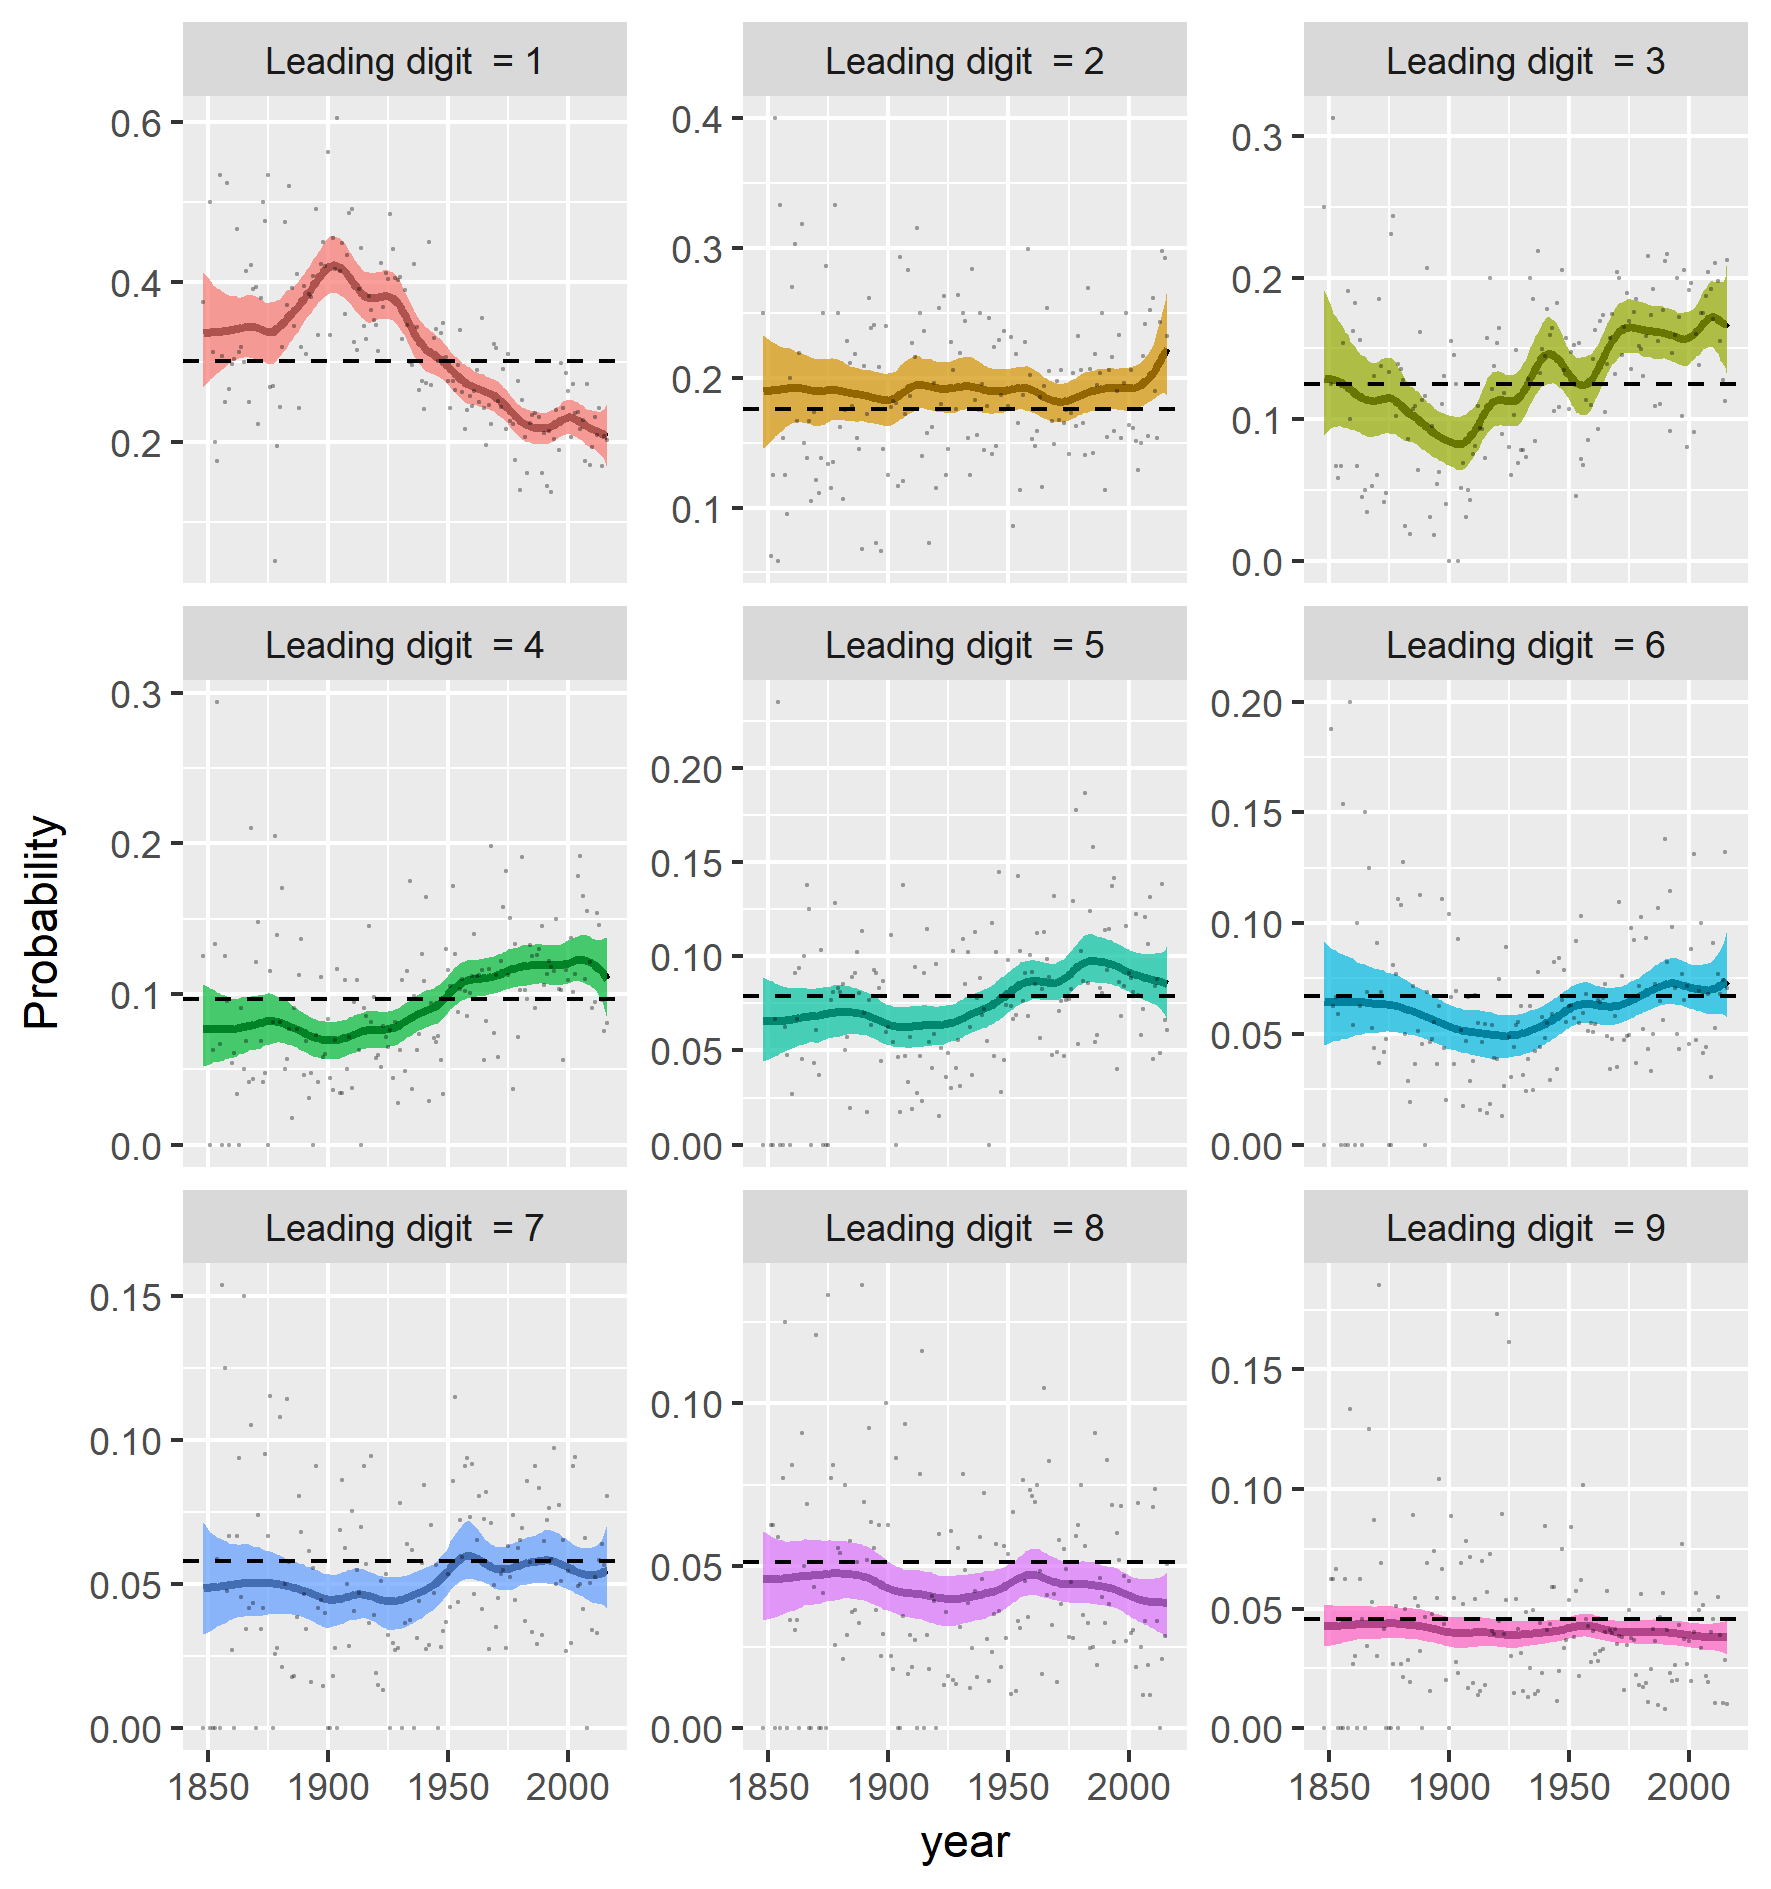
\includegraphics[width=1\linewidth]{Fig3}
\begin{center}
\vspace{-0.4cm}
\scriptsize Fig 4. \textbf{Dynamics of $(p_{1,t},\ldots,p_{9,t})$}\\ 
\end{center}
\begin{flushleft}
\vspace{-0.3cm}
\begin{myindentpar}{0.5cm}
\renewcommand{\baselinestretch}{0.8}
\scriptsize The posterior mean (solid line) and 95\%  credible bands (shaded area), the empirical distribution (point), and  Benford distribution (dashed line).
\end{myindentpar}
\end{flushleft}
\vspace{0.1cm}
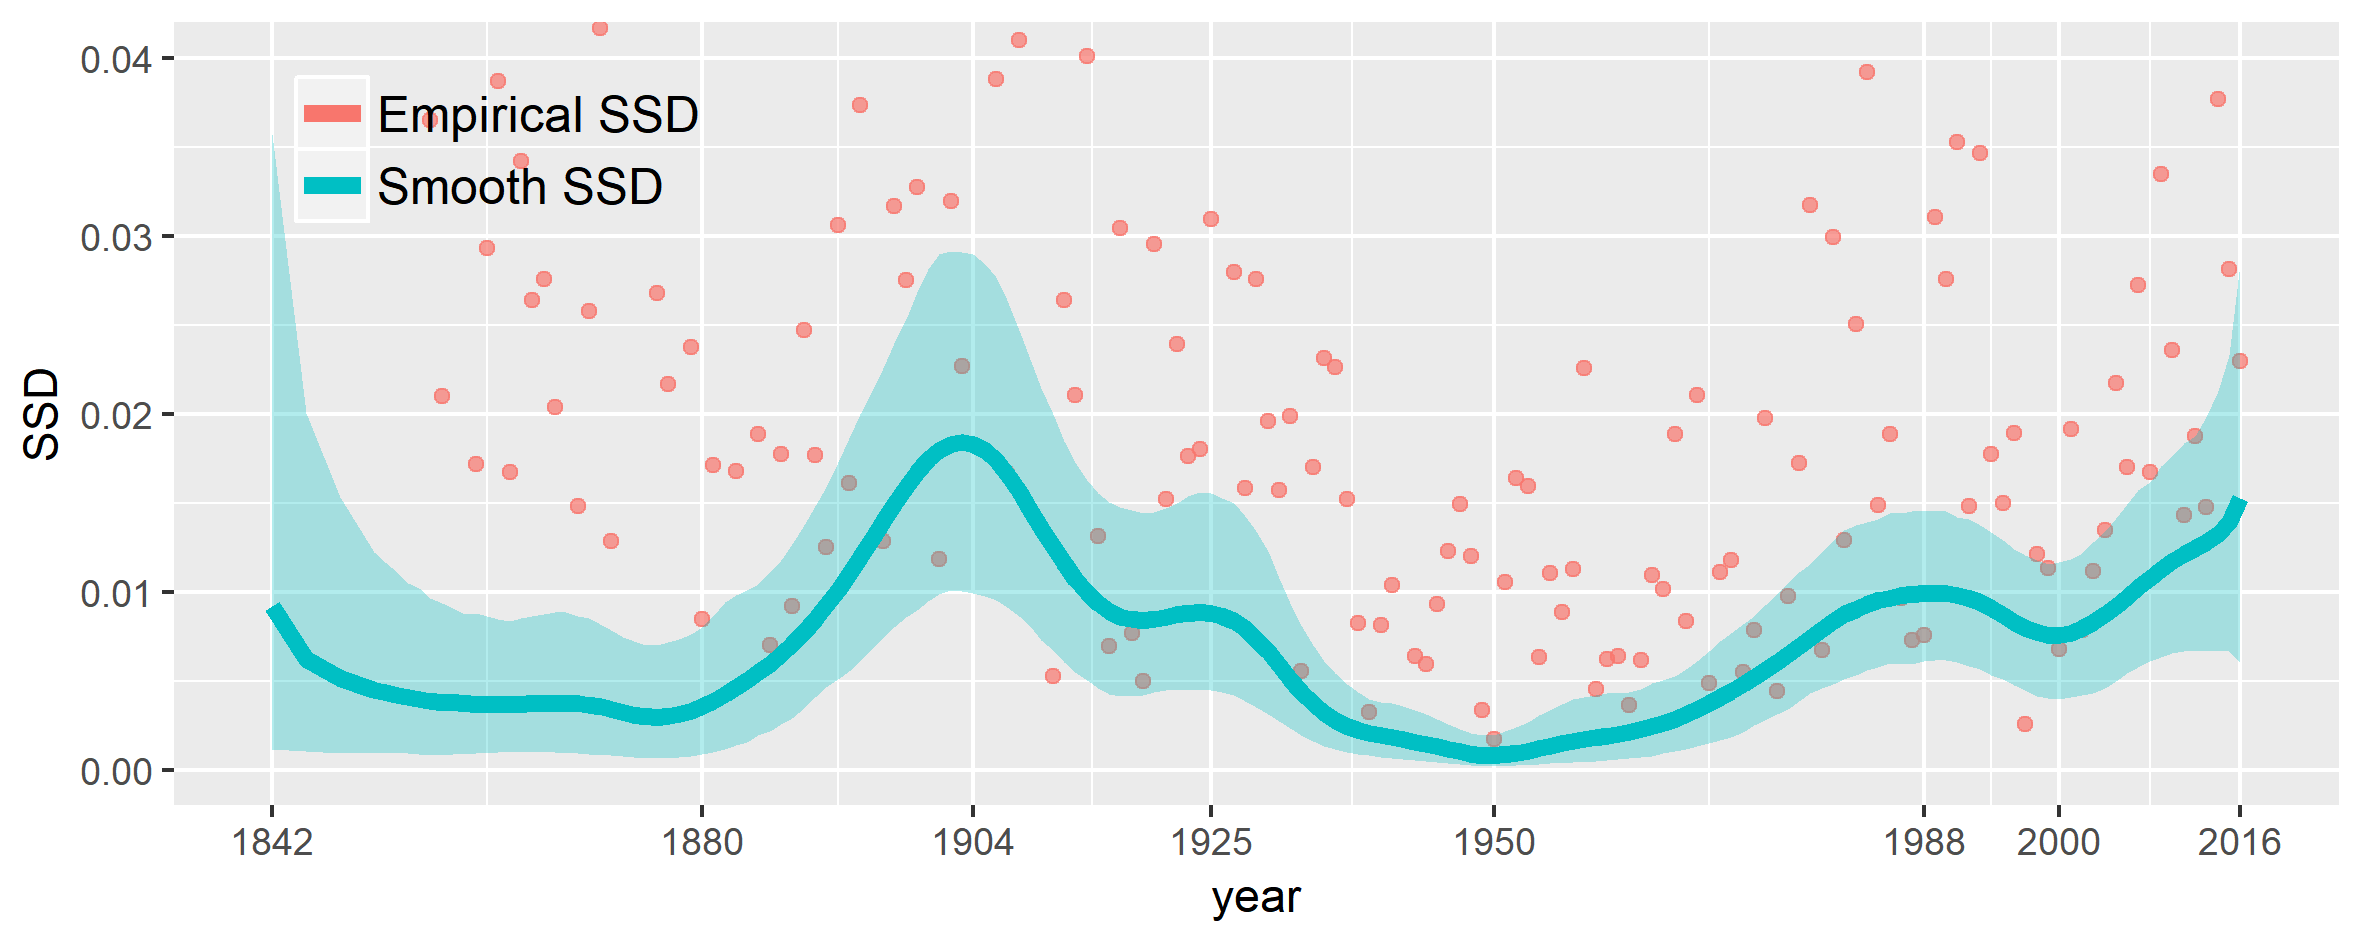
\includegraphics[width=1\linewidth]{Fig4}
\vspace{-0.8cm}
\begin{center}
\scriptsize Fig 5. \textbf{Homogeneity of GTC data}\\ 
\end{center}
\begin{flushleft}
\vspace{-0.2cm}
\begin{myindentpar}{0.5cm}
\renewcommand{\baselinestretch}{0.8}
\scriptsize The posterior mean of  SSD (solid blue line), 95\% credible bands (shaded blue area) and the empirical SSD (red point) in each year.
\end{myindentpar}
\end{flushleft}
\vspace{0.1cm}

\end{minipage}



}



\renewcommand{\baselinestretch}{1.0}

\headerbox{5. References}{name=references,column=2,span=1,below=application,above=bottom}{
\footnotesize % Reduce the font size in this block
\renewcommand{\section}[2]{\vskip 0.01em} % Get rid of the default "References" section title
\nocite{Hill1995} % Insert publications even if they are not cited in the poster
\bibliographystyle{unsrt}
\bibliography{mybib} % Use sample.bib as the bibliography file
}

\end{poster}

\end{document}
